\documentclass{beamer}
\usetheme{boadilla}


\usepackage{amsmath,amssymb,amsthm} 
\usepackage{caption}
\usepackage{gensymb}
\usepackage{preview}
\usepackage{bm}
\usepackage{mathtools}
\usepackage{hyperref} 
\usepackage{fancyhdr}
\usepackage{indentfirst}
\usepackage{tablefootnote}
%\usepackage{cmbright}
\usepackage[russian, english]{babel}
\usepackage[T1,T2A]{fontenc}
\usepackage[utf8]{inputenc}
\usepackage [autostyle, english = american]{csquotes}
\MakeOuterQuote{"}

\title{Clustering, Mixtures, and the EM Algorithm}
\subtitle{Machine Learning: Module 1}
\author{Sean Norton; Simon Hoellerbauer}
\begin{document}
\begin{frame}
	\titlepage
\end{frame}

\section{Cluster Analysis}

\begin{frame}
\frametitle{The Problem: Finding Groups}
	In social science, we often believe our observations have some sort of group structure.
	\begin{itemize}
		\item Regime types
		\item Types of voters
		\item Types of legislators		
	\end{itemize}
	However, our data doesn't (generally) come with these groupings conveniently pre-labeled.

\end{frame}

\begin{frame}
\frametitle{E.g. Regime Types}
	
	\begin{figure}
		\centering
		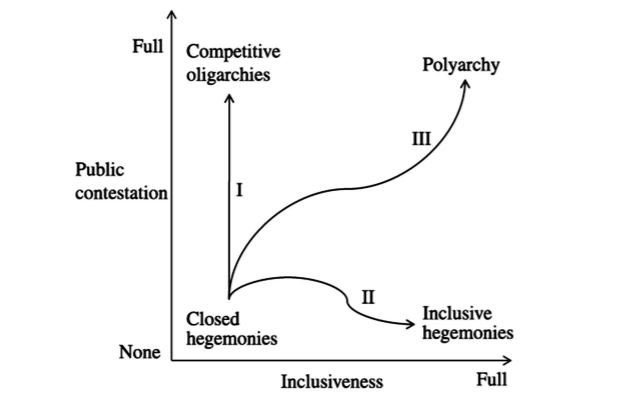
\includegraphics[width=0.7\linewidth]{dahl}
		\caption{Dahl: Regime Types}
		\label{fig:dahl}
	\end{figure}

\end{frame}

\begin{frame}
\frametitle{The Problem Continued}
	The general approach to dealing with this problem has been to hand-label cases. This is problematic because:
	\begin{itemize}
		\item It's time-consuming
		\item Humans aren't able to consider all available data at once
		\item It relies on researcher discretion
		\item For large datasets (e.g. all countries in the world), this is impossible.
	\end{itemize}
	What if there was a way to find latent groupings between our cases quickly and with as little researcher discretion as possible?
\end{frame}

\begin{frame}
\frametitle{Enter Cluster Analysis}
	This is exactly what cluster analysis is intended to do!\\
	Given:
	\begin{itemize}
		\item Data
		\item Number of clusters
		\item Variables
		\item Similarity measure
	\end{itemize}
	A cluster analysis algorithm finds groupings, or clusters, that maximize the similarity between observations within a cluster. 
\end{frame}

\begin{frame}
\frametitle{K-Means and Notation}
	One of the most common similarity measures is the squared distance between the center (mean) of a cluster. \\
	This is known as \textit{k-means} or \textit{k-nearest neighbor} clustering.\\
	Before we dive into the math, some notation:
	\begin{itemize}
		\item $k$: total number of clusters
		\item $r_{nk}$: indicator vector of cluster membership for observation $x_n$
		\item $\mu_k$: the centroid of cluster $k$
	\end{itemize}
\end{frame}

\begin{frame}
\frametitle{K-Means: The Math}
	Cluster analysis relies on a measure of similarity, which in k-means is:
	
	\begin{align*}
	J = \sum_{n=1}^{N}\sum_{k=1}^{K} r_{nk}  \| x_n - \mu_k \|^2
	\end{align*}
	This number $J$ is also known as a \textit{distortion measure}.\\
	What (hopefully) familiar thing does this measure look like?
\end{frame}

\begin{frame}
\frametitle{The Math cont.}
	\textbf{Q}: But how do we choose values of $\mu_k$ given that we don't actually know the cluster assignments?\\
	\textbf{A}: We don't!\\
	We can find $k_m$ through a version of the \textit{expectation-maximization algorithm}:
	\begin{enumerate}
		\item Initialize some random values for $\mu_k$
		\item Minimize $J$ w.r.t. $r_{nk}$; i.e. assign cluster memberships in order to minimize distortion
		\item Using the previous $r_{nk}$, minimize J w.r.t to $\mu_k$; i.e., assign new means that minimize distortion
		\item Repeat until convergence ($J$ does not change, or the change falls below some threshold)
	\end{enumerate}

\end{frame}

\begin{frame}
 \frametitle{The Math: Visualized}
 \begin{figure}
 	\centering
 	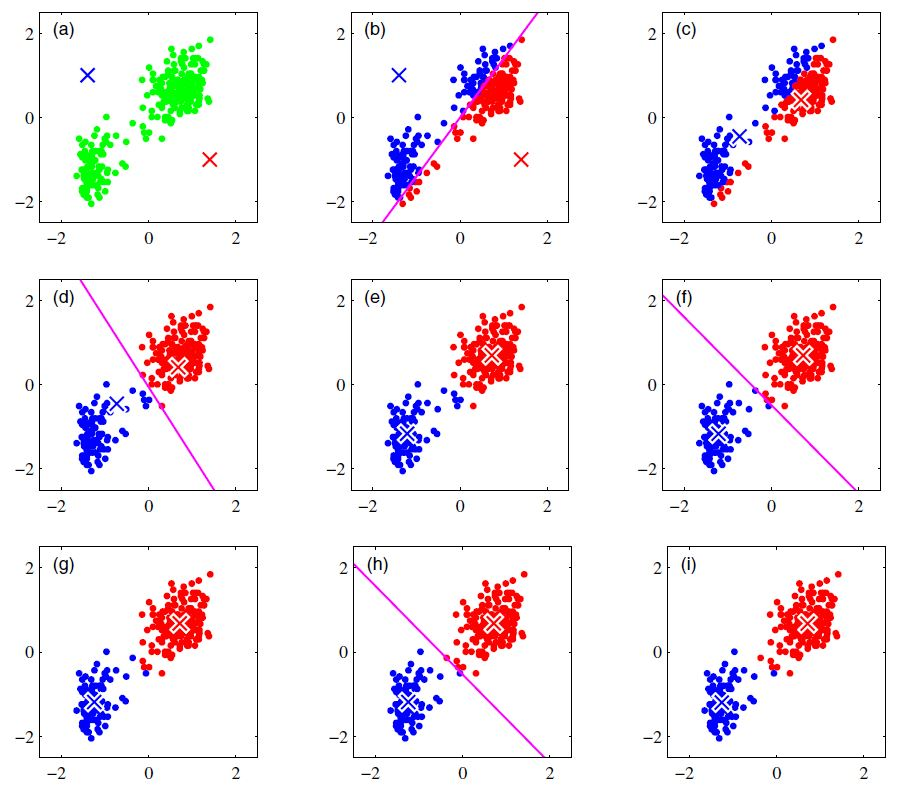
\includegraphics[width=0.7\linewidth]{bishopkmeans}
 	\caption{Optimizing Clusters}
 	\label{fig:bishopkmeans}
 \end{figure}
 
\end{frame}

\section{Clustering Problems}

\begin{frame}
	\frametitle{Problems with Clustering}
	\begin{itemize}
		\item Choosing $k$: this requires trying a lot of different $k$ w.r.t. some similarity measure
			\begin{itemize}
				\item Plot the WCSS against the number of clusters, and look for a "bend" in the plot; this is known as the elbow method
				\item Use average silhouette width: the silhouette is a measure how similar an observation is to its own cluster (consistency) and how dissimilar it is to other clusters (separation)
				\item Gap statistics: compare multiple values of $k$ to a simulated reference distribution of datasets with clusters varying from $k=1$ to $k=max$
			\end{itemize}
		\item Sensitivity to outliers; luckily, there are clustering methods other than $k$-means
			\begin{itemize}
				\item Partitioning around medoids (PAM): uses median instead of mean
				\item Hierarchical clustering: creates a tree-based representation of the data without specifying $k$; clusters are created by "cutting" the tree.  
			\end{itemize}
		\item Fundamentally descriptive; clusters will not necessarily be the same given different data
	\end{itemize}
\end{frame}

\begin{frame}
\frametitle{Problems cont.}

\begin{figure}
	\centering
	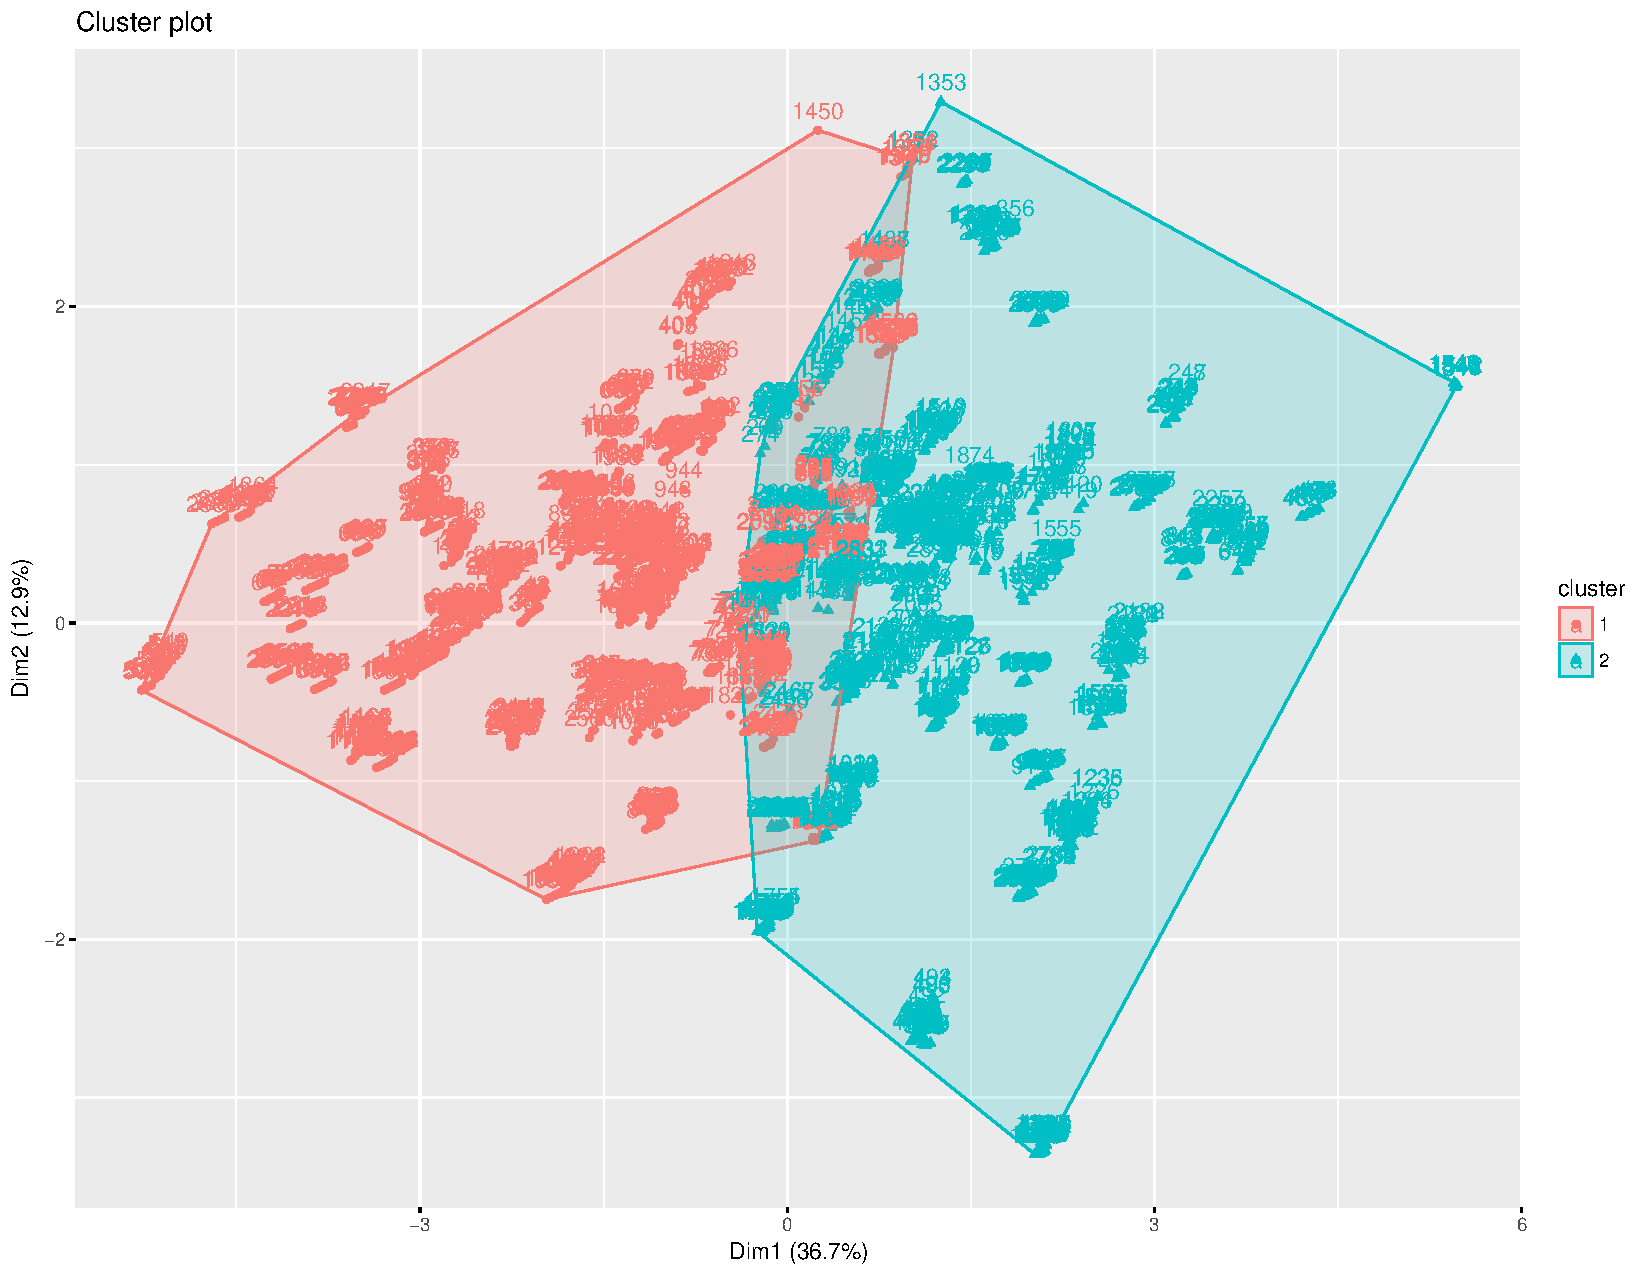
\includegraphics[width=0.7\linewidth]{clusterplot}
	\caption{My Cluster Plot}
	\label{fig:clusterplot}
\end{figure}

\end{frame}

\section{Mixture Models: Basics}

\begin{frame}
\frametitle{Mixture Models: Motivation}
	What if instead of "hard" cluster assignments, we could assign a probability that cases belong to a particular group?\\
	That is precisely what \textit{mixture models} are intended to do!\\
	Mixture models allow observations to belong to different distributions - either different parameterizations of the same distribution, or different distributions entirely.\\
	This allows us to:
	\begin{itemize}
		\item Sort cases into groups, much like cluster models, but do so in a way that quantifies uncertainty
		\item Estimate a model in the same step as the grouping, which most out-of-the-box clustering packages do not do
		\item Work with data that has a multimodal distribution without having to discard a substantial amount of variation. 
	\end{itemize}
\end{frame}

\begin{frame}
\frametitle{Motivating Example: Old Faithful}
	\begin{figure}
		\centering
		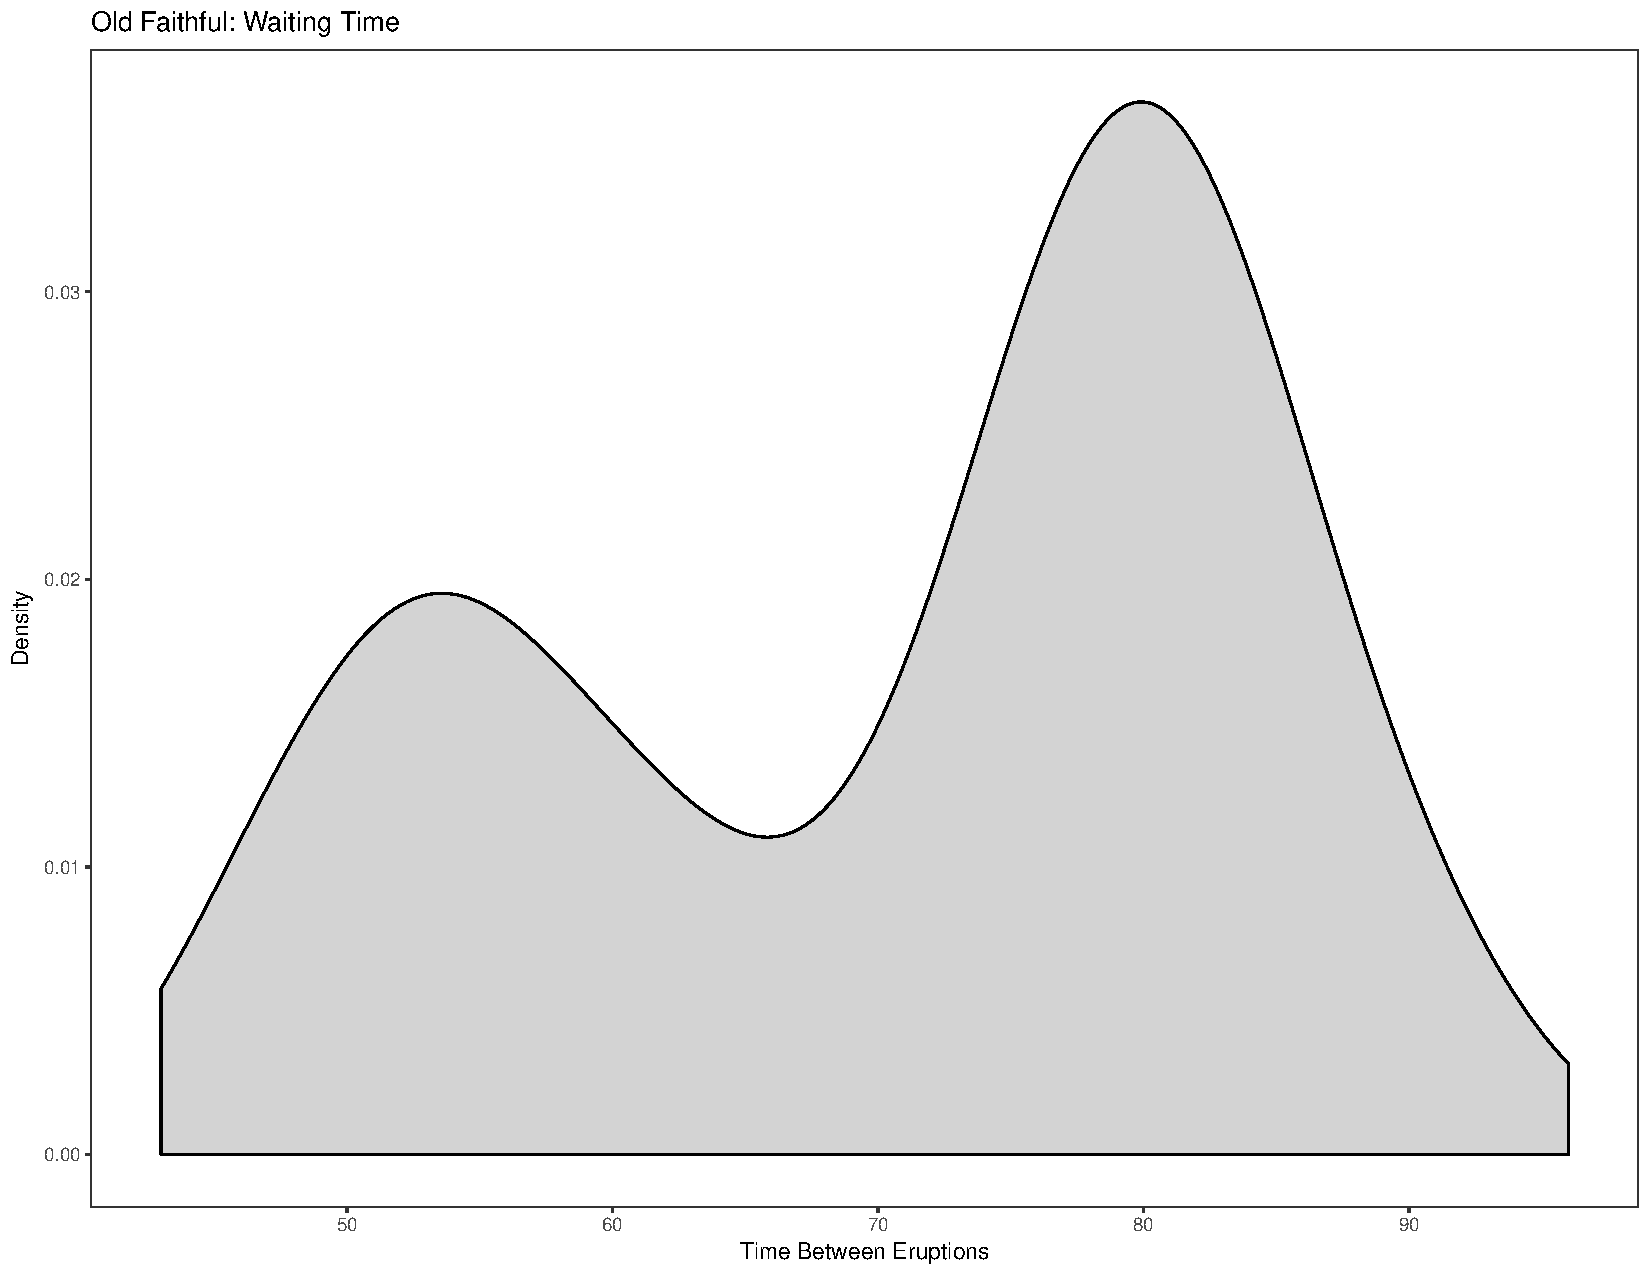
\includegraphics[width=0.7\linewidth,]{faithfulplot}
		\caption*{}
		\label{fig:faithfulplot}
	\end{figure}
	
\end{frame}

\begin{frame}
\frametitle{Motivating Example: Old Faithful}
Clearly, this data appears to be normally distributed, but not in a single normal distribution.\\
Instead of fitting a single Gaussian, we can fit a \textit{mixture} of Gaussians of the following form:
\begin{align*}
p(x) = \sum_{k=1}^{K} \pi_k \mathcal{N} (x | \mu_k, \Sigma_k)
\end{align*}
Where $\pi_k$ is the probability that an observation belongs to cluster $k$. \\
This is a Gaussian mixture model (GMM)
\end{frame}

\begin{frame}
\frametitle{Deriving the Model}
	To be able to estimate $\pi_k$, let us define a $K$-dimensional vector \textbf{z}, which is 1 if an observation is in group $k$ and 0 otherwise. \textbf{z} is a latent variable - deriving the model this way will be of use later.\\
	\begin{align*}
	p(z_k = 1) = \pi_k
	\end{align*}
	Or alternatively, since this is a 1-of-K vector:
	\begin{align*}
	p(\mathbf{z})  = \prod_{k = 1}^{K} \pi_k^{z_k}
	\end{align*}
	What must be true of $\mathbf{\pi}$

\end{frame}

 \begin{frame}
 \frametitle{Deriving the Model}
 
 	The conditional distribution $(\mathbf{x} | \mathbf{z})$ is then:

 	\begin{align*}
 	p(x|z) = \prod_{k = 1}^{K} \mathcal{N}(\mathbf{x} | \mu_k, \Sigma_k)^{z_k}
 	\end{align*}
 	
 	Marginalizing the distribution over $\mathbf{z}$ returns the original formulation:
 	
 	\begin{align*}
 	p(x) = \sum_{k=1}^{K} \pi_k \mathcal{N} (x | \mu_k, \Sigma_k)
 	\end{align*}
 	
 	While this seems like a useless exercise, we can now work with the joint distribution of our observations and the latent variable, $p(x|z)$, which will make estimation considerably easier.
 
 \end{frame}

\begin{frame}
\frametitle{More for Later}
Another important quantity for later will be $\gamma(z_k)$.\\
For now, think of $\pi_k$ as the \textit{prior} probability of group membership. We are also interested in the posterior probability ($p(z_k = 1|x) $), which can be calculated using Bayes' Rule:

\begin{align*}
  \frac{p(z_k = 1) p(x|z_k =1 )}{\sum_{j = 1}^{k} p(z_j = 1) p(x|z_j=1)}\\
\end{align*}

Do this terms look familiar? How would you put this in terms of the joint PDF we just derived?
\end{frame}

\begin{frame}
	\frametitle{Attempting Vanilla MLE}
	The log-likelihood of the GMM is given by:
	\begin{align*}
	ln\; p(x|\pi, \mu, \Sigma) = \sum_{n=1}^{N} ln\{\sum_{k=1}^{k} (x_n | \mu_k, \Sigma_k) \}
	\end{align*}
	What do you notice is strange about this log-likelihood compared to ones we've seen before?
\end{frame}

\begin{frame}
\frametitle{Attempting Vanilla MLE}
	In the log likelihood of the GMM, the logarithm does not act directly on the Gaussian distribution. When we set the derivatives of likelihood to $0$ in order to maximize the parameters, this results in there not being a closed form solution.
	
	\begin{align*}
	 0&= -\sum_{n=1}^{N} \gamma(z_{nk}) \Sigma_k(x_n - \mu_k)
	\end{align*}
	
	Where the mean of group $k$ is the mean of each observation in the group, weighted by the posterior probability of its membership in that group:
	\begin{align*}
		 \mu_k &= \frac{1}{N_k} \sum_{n=1}{N} \gamma(z_{nk})x_n \\
		 N_k &= \sum_{n=1} \gamma({z_{nk}}) = \text{\# of points in cluster k}
	\end{align*}
	
\end{frame}

\begin{frame}
\frametitle{Attempting Vanilla MLE}	
	Similarly, the covariance is given by:
	\begin{align*}
	\Sigma_k = \frac{1}{N_k} \sum_{n=1}{N} \gamma(z_{nk})(x_n - \mu_k)(x_n - \mu_k)^\intercal
	\end{align*}
	And the mixing coefficients are (intuitively):
	\begin{align*}
	\pi_k = \frac{N_k}{N}
	\end{align*}
\end{frame}

\begin{frame}
\frametitle{Problems with MLE}
\begin{itemize}
	\item As can be seen from the previous partial derivatives, the mean and variance of the GMM estimates depend on the posterior probabilities, which themselves depend on the mean and variance. Therefore, there is not a closed form solution.
	\item Because we now have multiple components, a situation can arise where a component collapses on a single point when an observation is equal to the component mean, contributing infinitely to the log likelihood:
	\begin{align*}
	&\mathcal{N}(x_n|\mu_k, \Sigma_j) = \frac{1}{2\pi^{\frac{1}{2}}}\frac{1}{\sigma_j}\\ 
	&\lim_{\sigma_j \to \infty} = \infty
	\end{align*}
\end{itemize}

\end{frame}

\begin{frame}
\frametitle{Problems with MLE}
	\begin{itemize}
		\item MLE also suffers from an \textit{identifiability} issue: in a $K$ component mixture, there are $K!$ possible solutions for assigning $K$ parameters to $K$ components; for any chosen parameter in the $\pi_k$ parameter space there are $k-1!$ points that produce the exact same distribution
		\item This creates a multimodal distribution of the log likelihood in which there is no unique solution; more generally for all latent variable models, this is known as \textit{label nonidentifiability}
	\end{itemize}
\end{frame}

\section{Expectation-Maximization Algorithm}

\begin{frame}
\frametitle{The Expectation-Maximization Algorithm}
	\begin{itemize}
		\item EM Algorithm allows us to approach MLE in a much easier way
		\item However, as we will come to see later, the EM algorithm---or a certain interpretation of it---can also be used in Bayesian analysis, either to retrieve the MAP parameter estimates, or to retrieve the entire posterior, with variational inference
		\item In general, we use it when we have latent variables (the collection of which, in line with terminology used with mixture models, is usually termed $\mathbf{Z}$)
		\item We will exploit the existence of these latent variables to make finding parameter and latent variables estimates easier
	\end{itemize}
\end{frame}

\begin{frame}
\frametitle{The Basics: Our Starting Point}
Given the former:	
	\begin{itemize}
		\item We have a probabilistic model where we term all observed variables as $\mathbf{X}$, all latent variables as $\mathbf{Z}$, and all parameters as $\boldsymbol{\theta}$
		\item We want to find the maximum likelihood estimates for 
		\begin{align}
			p(\mathbf{X}|\boldsymbol{\theta}) = \sum_{\mathbf{Z}}p(\mathbf{X},\mathbf{Z}|\boldsymbol{\theta}) 
		\end{align}
		Note: here we assume $\mathbf{Z}$ is discrete, but it doesn't have to be. What would change if it were continuous?
		\item Let us assume that $	p(\mathbf{X}|\boldsymbol{\theta})$ cannot be maximized as is, and that maximizing the \textbf{complete data likelihood} $p(\mathbf{X},\mathbf{Z}|\boldsymbol{\theta})$ is more straightforward. Note that, as Sean said, we will not be able to maximize even this function directly, because of the interdependence of parameters and latent variables. 
	\end{itemize}
\end{frame}

\begin{frame}
\frametitle{The Basics: Oh Goodness, This Isn't So Basic Anymore}
Then let there be a distribution $q(\mathbf{Z})$ defined over the latent variables. For any choice of this distribution, it can be shown that
		\begin{align}
			\text{ln}p(\mathbf{X}|\boldsymbol{\theta}) =\mathcal{L}(q, \boldsymbol{\theta}) + \text{KL}(q\|p)
		\end{align}
where
		\begin{align}
			\mathcal{L}(q, \boldsymbol{\theta}) = \sum_{\mathbf{Z}}q(\mathbf{Z})\text{ln}\bigg\{\frac{p(\mathbf{X,  Z}|\boldsymbol{\theta})}{q(\mathbf{Z})}\bigg\} \label{eq:2}
		\end{align}
and
	\begin{align}
		\text{KL}(q\|p) = - \sum_{\mathbf{Z}}q(\mathbf{Z})\text{ln}\bigg\{\frac{p(\mathbf{Z|  X},\boldsymbol{\theta})}{q(\mathbf{Z})}\bigg\}
	\end{align}
\end{frame}

\begin{frame}
\frametitle{The Basics: Functionals + Lower Bound of Marginal Likelihood}
\begin{itemize}
	\item Note that w.r.t the distribution $q(\mathbf{Z})$, $\mathcal{L}(q, \boldsymbol{\theta})$ is a \textit{functional}, that is, ``an operator that takes a function .... and returns and output value'' (Bishop 2006, 703). The ``value'' that maximizes a functional is a function. This idea is especially important in variational inference, which is built on the calculus of variations. W.r.t to $\theta$, $\mathcal{L}(q, \boldsymbol{\theta})$ is a function. 
	\item Note also that $\text{KL}(q\|p)$ is the Kullback-Leibler divergence between our distribution $q(\mathbf{Z})$ and the posterior distribution $p(\mathbf{Z}|\mathbf{X}, \boldsymbol{\theta})$.
	\item Because $\text{KL}(q\|p) \geq 0$, equalizing $0$ iff $q(\mathbf{Z}) = p(\mathbf{Z}|\mathbf{X}, \boldsymbol{\theta})$, this implies that $\mathcal{L}(q, \boldsymbol{\theta}) \leq \text{ln}p(\mathbf{X}|\boldsymbol{\theta})$
	\item $\mathcal{L}(q, \boldsymbol{\theta})$ turns out to be the lower bound of 		$\text{ln}p(\mathbf{X}|\boldsymbol{\theta})$.  
\end{itemize}

\end{frame}

\begin{frame}
\frametitle{Decomposition in Picture Form}
 \begin{figure}
	\centering
	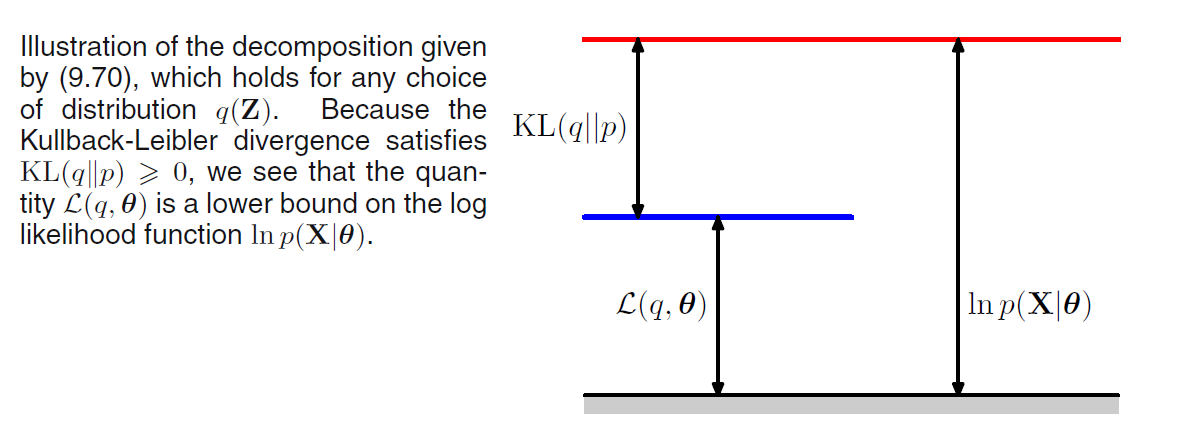
\includegraphics[width=0.7\linewidth]{decomposition}
	\caption{Illustration of Decomposition of $	\text{ln}p(\mathbf{X}|\boldsymbol{\theta})$}
	
	\textit{Source:} Bishop (2006), pg. 451
	\label{fig:decomposition}
\end{figure}
\end{frame}

\begin{frame}
\frametitle{The Basics: The Steps}
The EM algorithm is an algorithm with four steps, two of which are iterative:
	\begin{enumerate}
		\item We pick initial values for $\boldsymbol{\theta}^{old}$
		\item In the E Step, using these initial values for $\theta$, we maximize the lower bound $\mathcal{L}(q, \boldsymbol{\theta}^{old})$ described in the previous slide, with respect to the function $q(\mathbf{Z})$. That is to say, we hold the $\theta$'s fixed and allow only the distributional form of $q(\mathbf{Z})$ to vary. This produces a new distribution $\mathcal{L}(q, \theta)$. 
		\item In the M Step, we maximize this function with respect to the parameters $\boldsymbol{\theta}$, while holding $q(\mathbf{Z})$ constant. This produces new parameters $\boldsymbol{\theta}^{new}$.
		\item We repeat Steps 2 and 3 (the E and M Steps) until some convergence criteria is satisfied. In other words, $\boldsymbol{\theta}^{new}$ becomes the $\theta$ that are fixed in Step 2, and so on. 
	\end{enumerate}
\end{frame}

\begin{frame}
\frametitle{The Particulars: Something to Note}
	\begin{itemize}
		\item The EM algorithm is often described as having just two steps, but it is important to realize that it must be initialized (the choice of initial values can have consequences) and that you have to have some convergence tolerance, otherwise the algorithm could run forever. In addition, there are various convergence criteria that could be used.  
	\end{itemize}
\end{frame}

\begin{frame}
\frametitle{The Particulars: Where Does the Expectation Come In?}
\begin{itemize}
	\item Although E stands for expectation, this is something of a misnomer. You are really finding the distribution $q(\mathbf{Z})$ that maximizes the lower bound of the true ``likelihood'' (and in turn reduces the KL divergence between $q(\mathbf{Z})$ and $p(\mathbf{Z}|\mathbf{X}, \boldsymbol{\theta}^{old})$ to 0) when the parameters are fixed at a certain value. This really means that you are finding the parameters that make up this function. 
	\item It turns out that, because it drives the KL divergence to 0, this distribution $q(\mathbf{Z}) = p(\mathbf{Z}|\mathbf{X}, \boldsymbol{\theta}^{old})$.
	\item If we substitute this into \ref{eq:2}, we see that after the E step
	\begin{align*}
		\mathcal{L}(q,\boldsymbol{\theta}) = \sum_{\mathbf{Z}}p(\mathbf{Z}|\mathbf{X}, \boldsymbol{\theta}^{old})\text{ln}p(\mathbf{Z},\mathbf{X}| \boldsymbol{\theta}) - \sum_{\mathbf{Z}}p(\mathbf{Z}|\mathbf{X}, \boldsymbol{\theta}^{old})\text{ln}p(\mathbf{Z},\mathbf{X}| \boldsymbol{\theta}^{old})
	\end{align*}
	When it comes to taking the M step, we are optimizing this function w.r.t $\boldsymbol{\theta}$. As there are no $\boldsymbol{\theta}$'s in the second half of the function, this part is treated as a constant.
\end{itemize}
\end{frame}

\begin{frame}
\frametitle{The Particulars: Where Does the Expectation Come In?}
\begin{itemize}
	\item We then note that $\sum_{\mathbf{Z}}p(\mathbf{Z}|\mathbf{X}, \boldsymbol{\theta}^{old})\text{ln}p(\mathbf{Z},\mathbf{X}| \boldsymbol{\theta})$ is just the expectation of the complete data log-likelihood.
	\item This function is termed, in alternative formulations of the EM algorithm, $\mathcal{Q}(\boldsymbol{\theta}, \boldsymbol{\theta}^{old})$
	\item If we think through this, we can see that the E step, if we take a few shortcuts, just requires us to calculate the expectation of the complete data log-likelihood, which we then maximize in the M step. This explains the names---but we should recognize that there is a lot more going on in the background!   
\end{itemize}
\end{frame}

\begin{frame}
\frametitle{E-Step in Picture Form}
 \begin{figure}
	\centering
	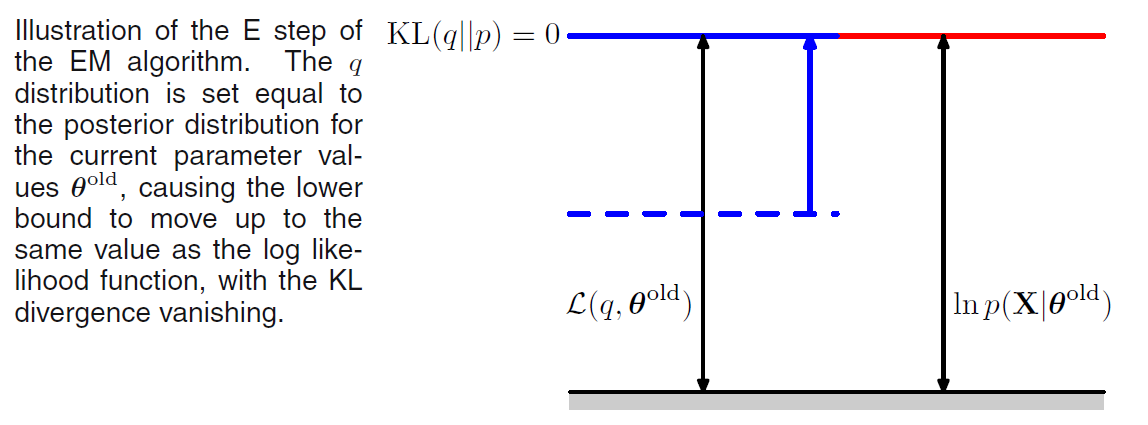
\includegraphics[width=0.7\linewidth]{e_step}
	\caption{Visualization of E Step}
	
	\textit{Source:} Bishop (2006), pg. 452
	\label{fig:e_step}
\end{figure}
\end{frame}

\begin{frame}
\frametitle{M-Step in Picture Form}
 \begin{figure}
	\centering
	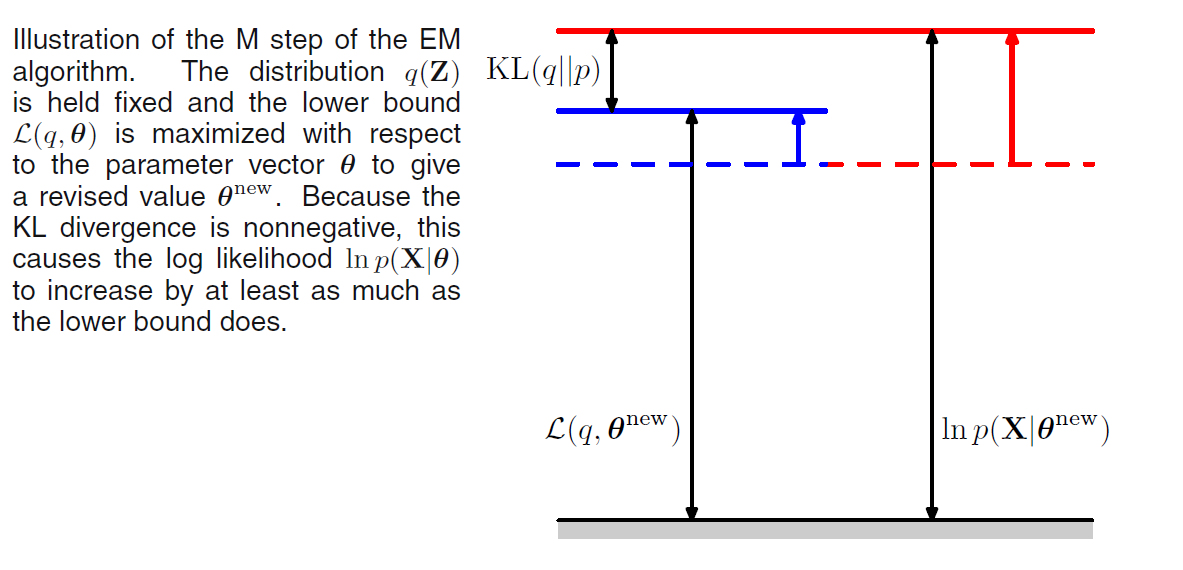
\includegraphics[width=0.7\linewidth]{m_step}
	\caption{Visualization of M Step}
	
	\textit{Source:} Bishop (2006), pg. 452
	\label{fig:m_step}
\end{figure}
\end{frame}

\begin{frame}
\frametitle{Putting it All Together in Picture Form}
 \begin{figure}
	\centering
	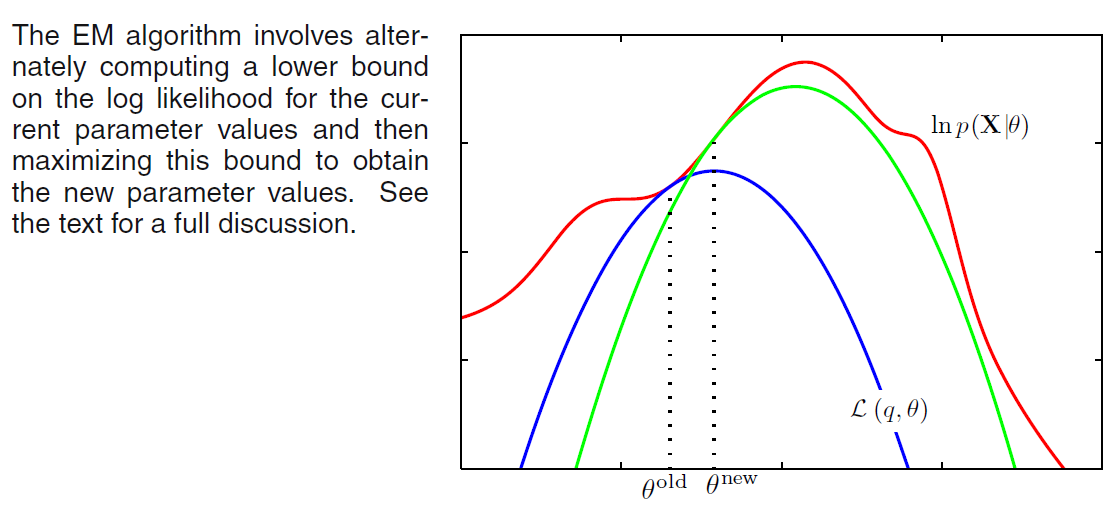
\includegraphics[width=0.7\linewidth]{em_algorithm}
	\caption{Visualization of EM Algorithm Process}
	
	\textit{Source:} Bishop (2006), pg. 453
	\label{fig:em_algorithm}
\end{figure}
\end{frame}

\begin{frame}
\frametitle{The Particulars: The Intuition Behind Why The EM Monotonically Increases The Observed Data Log-Likelihood}
As was shown in the previous slides, due to fact that $\mathcal{L}(q, \boldsymbol{\theta})$ is a lower bound on the , as we iterate the following string of inequalities becomes apparent:
\begin{align}
	\text{ln}p(\mathbf{X}|\boldsymbol{\theta}^{t}) = \mathcal{L}(q, \boldsymbol{\theta}^{t}) \leq \text{ln}p(\mathbf{X}|\boldsymbol{\theta}^{t+1}) = \mathcal{L}(q, \boldsymbol{\theta}^{t+1}) \leq \text{ln}p(\mathbf{X}|\boldsymbol{\theta}^{t+2})
\end{align}
In short, in each E step, we bring the lower bound as close as possible to the log likelihood. In each M step, we poke the log likelihood a bit further up the hill.\\

This means that we are steadily increasing the log likelihood, and we keep doing so until the increases get so small that they are indistinguishable from zero---and that's what we call convergence, folks! \textbf{Calculating the log likelihood is a good way to catch errors and bugs: if it decreases, something has gone wrong.}
\end{frame}

\begin{frame}
\frametitle{Issues with the MLE Version of EM Algorithm}
	\begin{itemize}
		\item As it has been explained here, we are still just doing MLE, really, as we are still just climbing a hill
		\item MLE can overfit
		\item MLE can fall into local maxima trap and is not guaranteed to find global maxima
		\begin{itemize}
			\item The EM algorithm needs to be initialized, so need to be careful with initial values, might have to start over various times
		\end{itemize}
		\item In particular, when it comes to Gaussian Mixture Models, MLE EM can find singularities, which is when a component has zero variance and a mean equal to one of the data points
	\end{itemize}
\end{frame}

\begin{frame}
\frametitle{Not Just MLE}
	\begin{itemize}
		\item This brings us to the important realization that EM is just an algorithm
		\item There are various ways of approaching it as a whole and the two steps individually
		\item For example, in order to help with the issue identified in the previous slide, can take a more Bayesian approach and use MAP. 
		\begin{itemize}
			\item Simply add the log prior to the complete data log-likelihood
			\item This does not change the E step and only impacts the M step
		\end{itemize}
		\item It is also possible to go ``fully Bayesian,'' which will lead us to variational inference! 
	\end{itemize}
\end{frame}

\section{EM For Gaussian Mixture Models}

\begin{frame}
\frametitle{EM for Gaussian Mixture Models}
We can apply the above discussion to find relatively easy parameter estimates for Gaussian Mixture Models in the following way:
	\begin{enumerate}
		\item Choose initial values for means $\boldsymbol{\mu}_k$, covariances $\boldsymbol{\Sigma}_{k}$, and mixing coefficients $\pi_k$
		\item E Step: Using these parameter values, determine the posterior probability of membership for each observation (also known as \textit{responsibilities}, as mentioned earlier), with the following equation:
		\begin{align}
			\gamma(z_{nk}) = \frac{\pi_k\mathcal{N}(x_n|\boldsymbol{\mu}_k, \boldsymbol{\Sigma}_k)}{\sum_{j = 1}^K \pi_j\mathcal{N}(x_n|\boldsymbol{\mu}_j, \boldsymbol{\Sigma}_j)}
		\end{align} 
		This equation can be derived from the expected complete data log-likelihood. See page 351 of Murphy (2012). 
	\end{enumerate}
\end{frame}

\begin{frame}
\frametitle{EM for Gaussian Mixture Models}
\begin{enumerate}
	\setcounter{enumi}{2}
	\item M Step: Using the responsibilities calculated in the E-Step, re-estimate the parameters. This will involve maximizing the expected complete data log-likelihood w.r.t each of the parameters in turn. The common thread that runs through the maximizing values is the responsibilities:
	\begin{align}
		\pi_k^{new} &= \frac{N_k}{N}\\
		\boldsymbol{\mu}_k^{new} &= \frac{1}{N_k}\sum_{n=1}^N\gamma(z_{nk})x_n\\
		\Sigma_k &= \frac{1}{N_k} \sum_{n=1}{N} \gamma(z_{nk})(x_n - \mu_k^{new})(x_n - \mu_k^{new})^\intercal
	\end{align}
	With 
	\begin{align}
		N_k &= \sum_{n=1} \gamma({z_{nk}}) = \text{\# of points in cluster k}
	\end{align}
	You've seen these already; we discussed them when we first talked about GMM. 
\end{enumerate}
\end{frame}

\begin{frame}
\frametitle{EM for Gaussian Mixture Models}
\begin{enumerate}
	\setcounter{enumi}{3}
	\item Evaluate the log likelihood in order to be able to check convergence and for errors and bugs in the code. You can also check for convergence within the parameters themselves. If convergence has not been reached, return to Step 2 (the E Step). 
\end{enumerate}
\end{frame}



\section{Beyond GMM}

\begin{frame}
\frametitle{Non-Gaussian Mixtures}
	Mixture models can be generalized to fit any distribution:
	\begin{align*}
	p(x) = \sum_{k=1}^{K} \pi_k p (x | \theta)
	\end{align*}
	
	Or even to mix \textit{different} distributions:
	
	\begin{align*}
	p(x) = \sum_{k=1}^{K} \pi_k p (x | z_i = k, \theta)
	\end{align*}
	
	Or even mixtures of non-parametric distributions - the mixing coefficient places no restrictions on the form of the distribution after it. 

\end{frame}

\begin{frame}
\frametitle{Mixtures of Bernoullis}
	Another common mixture is a mixture of Bernoulli distributions, also called \textit{latent class analysis}.\\
	As a reminder, the Bernoulli distribution is:
	\begin{align*}
	p(x|\mu) = \prod_{n = 1}^{N} \mu_i^{x_i}(1 - \mu_i)^{x_i}
	\end{align*}
	
	And a mixture of Bernoullis is:
	
	\begin{align*}
		p(x|\mu, \pi) = \sum_{k=1}^{K}p(x|\mu_k) 
	\end{align*}
\end{frame}


\begin{frame}
\frametitle{Mixtures of Bernoullis}
	This yields the following expressions of the mean and variance:
	\begin{align*}
	\mathbb{E}(x)& = \sum_{k=1}^{K} \pi_k \mu_k \\
	cov[x]  &= \sum_{k=1}^{K}  \pi_k (\Sigma_k + \mu_k \mu_k^{\intercal}) - \mathbb{E}(x)\mathbb{E}(x)^{\intercal}
	\end{align*}
	Where $\Sigma_{k}$ is the variance of a single Bernoulli component.\\
	What do you notice about the variance? How is this an improvement on a single Bernoulli?
\end{frame}

\begin{frame}
\frametitle{Mixtures of Bernoullis}
	The log likelihood is then:
	\begin{align*}
	ln p(\mathbf{X}|\mathbf{\mu}, \mathbf{\pi}) = \sum_{n=1}^{N} ln (\sum_{k =1}^{K} \pi_k p(x_n|\mu_k))
	\end{align*}
	Does this produce a closed form solution?\\
	Like GMM, does this have the potential to produce a singularity? Why or why not?
\end{frame}

\begin{frame}
\frametitle{EM with LCA}
	To use the EM algorithm on a mixture of Bernoulli's, we again introduce $z$ as latent mixture assignment. The conditional distribution $p(x|z, \mu)$ is then:
	\begin{align*}
	p(x|z, \mu) = \sum_{k=1}^{K} p(x|\mu_k)^{z_k}
	\end{align*}
	And the prior for $z$:
	\begin{align*}
	p(z|\mu) = \sum_{k=1}^{K} \pi_k^{z_k}
	\end{align*}
	Just like with the GMM, if we take the product of the conditional and the prior then marginalize out $z$, we get the original formulation back.
\end{frame}

\begin{frame}
\frametitle{EM with LCA}
	This then yields the complete-data log likelihood:
	\begin{align*}
	ln p(\mathbf{X}, \mathbf{Z}|\mathbf{\mu}, \mathbf{\pi}) = \sum_{n=1}^{N}\sum_{k=1}^{K} z_{nk} \{ln \pi_k + \sum_{i=1}^{D}[x_{ni} ln \mu_{ki} + (1 - x_{ni})ln(1-\mu_{ki})]\}
	\end{align*}
	How do we derive the E step from the complete data likelihood?
\end{frame}

\begin{frame}
\frametitle{EM with LCA}
	The E step evaluates the expectation for the latent variables w.r.t to the posterior distribution of $\mathbf{Z}$:
	\begin{align*}
	\mathbb{E}_{\mathbf{Z}}(.) = \gamma(z_{nk})\{ln \pi_k + \sum_{i=1}^{D}[x_{ni} ln \mu_{ki} + (1 - x_{ni})ln(1-\mu_{ki})]\}
	\end{align*}
	Where, just like with the GMM, the posterior is calculated using Bayes' rule:
	\begin{align*}
	\gamma(z_{nk}) =  \frac{\pi_k p(x_n|\mu_k)}{\sum_{j =1}^{K} \pi_j p(x_n | \mu_j)}
	\end{align*}
	What does the M step do after this?

\end{frame}

\begin{frame}
\frametitle{Putting It All Together}
This suggests a generalized way to put together any mixture model for estimation with EM:
\begin{enumerate}
	\item Create a PDF, $p(x)$, that includes a mixing coefficient $\pi$
	\item Re-conceptualize that PDF in terms of a latent variable, $z$
	\item Find the complete data log-likelihood
	\item Take the expectation of step 3 w.r.t.  to $Z$
	\item Calculate the expression of the posterior of $Z$ using Bayes' rule.
	\item Run the EM algorithm, and hopefully get interesting results!
\end{enumerate}
Extra credit question: if you write your own EM algorithm based on the above, how can you check that it's working properly?
\end{frame}

\end{document}
